\documentclass[12pt,titlepage]{article}

\usepackage{amsmath,amsthm}
\usepackage{unicode-math}
\usepackage{xltxtra}
\usepackage{xgreek}

\setmainfont{Times New Roman}

\usepackage{tabularx}

\usepackage[table]{xcolor}
\usepackage{tikz}
\pagestyle{empty}

\usepackage{geometry}
 \geometry{a4paper, top=53mm, bottom=53mm, left=40mm, top=40mm}

 \usepackage{graphicx}


 \usepackage{wrapfig}

 \renewcommand{\baselinestretch}{1.5}

 \newtheorem{proposition}{Πρόταση}
 \newtheorem{corollary}{Πόρισμα}


 \usepackage{hyperref}
%%\address{Ερυθραίας 46\\ 54351 Θεσσαλονίκη}

\begin{document}

\begin{titlepage}
 \begin{center}
  \Huge {Η Πίεση και τα Μαθηματικά της}

  \vspace{1.5cm}
  \Large {Μαθηματικά και οι άλλες επιστήμες στην εκπαίδευση}
 \end{center}
 \vspace{2cm}
 \begin{center}

  \begin{tabular}{ c c c }
   \Large{Κωνσταντίνος} & \Large{Παναγιώτης} & \Large{Μάριος} \\
   \Large{Λόλας} & \Large{Πετρίδης} & \Large{Ελευθεριάδης} \\
   \textit{Ερυθραίας 46,} & \textit{Δαγκλή 45,} & \textit{Αργοναυτών 41} \\
   \textit{Θεσσαλονίκη} & \textit{Τριανδρία} & \textit{Καλαμαριά} \\
   τηλ.6973380837 & τηλ.6973416317 & τηλ.6937201887 \\
   costasmath@yahoo.gr & sch@sch.gr & marioelef@gmail.com \\
  \end{tabular}

  \vspace{2cm}
  \textbf{Περίληψη}

  Αν υπήρχε η διαίρεση διανυσμάτων, η πίεση ορισμένη ως $p=\vec{F}/\vec{A}$ θα ήταν μία "εύκολη" έννοια. Εκεί ακριβώς μπλέκονται τα πράγματα ως προς την φύση της πίεσης ώντας διανυσματικό ή μη μέγεθος και κυρίως πώς μπορεί να μελετηθεί και να ερμηνευτεί από την μαθηματική της σκοπιά με σκοπό να γίνει πλήρως κατανοητή από μαθητές και όχι μόνο.

 \end{center}

\end{titlepage}

\section{Η πίεση στη Φυσική}
Στο σχολικό βιβλίο Φυσικής της Β Γυμνασίου\textsuperscript{\cite{fysikiB}}, η πίεση ορίζεται ως "\textit{το πηλίκο της δύναμης που ασκείται κάθετα σε μια επιφάνεια προς το εμβαδόν της επιφάνειας αυτής.}", δηλαδή
\begin{equation} \label{eq:1}
 p=\frac{\vec{F}}{A}
\end{equation}
Στην επόμενη παράγραφο ξεκαθαρίζει λέγοντας ότι η πίεση "\textit{δεν είναι διανυσματικό μέγεθος}", αλλά αμέσως μετά στην επόμενη πρόταση, αναφέρει ότι "\textit{εκφράζει την δύναμη που ασκείται κάθετα στη μονάδα επιφάνειας}". Έχουμε λοιπόν από την μία την δύναμη, η οποία είναι διάνυσμα και από την άλλη την επιφάνεια. Αυτό προκαλεί μία σύγχηση ως προς τη φύση της πίεσης ως μέγεθος διανυσματικό ή μονόμετρο. Εκεί βέβαια σταματάει και η συζήτηση στην τάξη αφού οι μαθητές δεν φαίνεται να αναρωτιούνται τι ακριβώς συμβαίνει.

Βέβαια σε έναν μαθητή της Β Γυμνασίου δεν μπορούμε να εξηγήσουμε όλες τις πράξεις των διανυσμάτων, γι' αυτό και το παρόν άρθρο αναφέρεται σε μαθητές τουλάχιστον Β Λυκείου. Στην Β Λυκείου, οι εν λόγω μαθητές στα Μαθηματικά προσανατολισμού διδάσκονται πράξεις μεταξύ διανυσμάτων και πιο συγκεκριμένα την πρόσθεση, την αφαίρεση, το βαθμωτό γινόμενο με πραγματικό αριθμό και το εσωτερικό γινόμενο.

Έτσι λοιπόν στην Φυσική Γ Λυκείου\textsuperscript{\cite{fysikiG}} με την νέα ύλη στην οποία προστέθηκαν και τα ρευστά λογικά θα πρέπει να έχει ξεκαθαριστεί πλήρως η έννοια της πίεσης.

\section{Διαισθητική Προσέγγιση}

Αν βυθίσουμε ένα μανόμετρο σε υγρό σε συγκεκριμένο βάθος, θα διαπιστώσουμε ότι περιστρέφοντας το, η πίεση δεν μεταβάλεται. Έτσι η λογική επιβάλει το συμπέρασμα ότι η πίεση δεν έχει κατεύθυνση, συνεπώς είναι μονόμετρο μέγεθος\textsuperscript{\cite{Halliday1}}.

\section{Μαθηματική Προσέγγιση}
Αν θεωρήσουμε μόνο την εξίσωση (\ref{eq:1}), η πίεση θα έπρεπε να είναι διανυσματικό μέγεθος, αφού
\begin{equation} \label{eq:4}
 p=\vec{F}\cdot\frac{1}{A}
\end{equation}
και ο βαθμωτός πολλαπλασιασμός ως γνωστόν ορίζεται ως $\mathbb{R} \times V \to V$. Το λάθος στον τύπο (\ref{eq:1}) είναι ότι η επιφάνεια δεν είναι μονόμετρο μέγεθος, αλλά διανυσματικό. Ο λόγος είναι ότι θέλουμε τη δύναμη που ασκείται κάθετα στην επιφάνεια, άρα δανειζόμαστε το κάθετο διάνυσμα $\vec{n}$ σε αυτή. Με άλλα λόγια $\vec{Α}=\vec{n}Α$ και ο τύπος στην πραγματικότητα είναι ο:
\begin{equation} \label{eq:2}
 p=\frac{\vec{F}}{\vec{A}}
\end{equation}

Πλέον είναι φανερό το πρόβλημα. Ίσως είναι το πρώτο μέγεθος το οποίο ορίζεται με φυσικό τρόπο ως πηλίκο δύο διανυσμάτων. Το εύκολο θα ήταν αν το παράγωγο μέγεθος ήταν η δύναμη $\vec{F}$, όπου τότε:
\begin{equation} \label{eq:3}
 \vec{F}=p\cdot \vec{A}
\end{equation}

Η πίεση έτσι δεν μπορεί να είναι τίποτα διαφορετικό από έναν πραγματικό αριθμό και η εξίσωση (\ref{eq:3}) είναι απλός βαθμωτός πολλαπλασιασμός. Η προηγούμενη εξίσωση εξηγεί πλήρως το μέτρο και την κατεύθυνση της δύναμης $\vec{F}$ που ασκείται σε τοίχωμα αν από την μεριά του υλικού η πίεση είναι $p$.

Η προηγούμενη παρατήρηση βασικά δικαιολογεί μάλλον και το γεγονός ότι η πίεση δεν ορίστηκε απλά ως "\textit{το πηλίκο του \textbf{μέτρου μίας κάθετης δύναμης} σε μία επιφάνεια ως προς το εμβαδό της επιφάνειας αυτής}". Αυτός ο ορισμός ενώ δικαιολογεί πλήρως την φύση της πίεσης ως μονόμετρο μέγεθος, του λείπει το φυσικό αποτέλεσμα όπως αυτό εκφράζεται από την εξίσωση (\ref{eq:3}).

\section{Μια πιο Μαθηματική Προσέγγιση}

Ενώ φαίνεται να έχει εγκαταληφθεί η προσέγγιση της πίεσης ως πηλίκο διανυσμάτων από εκπαιδευτικούς, ίσως θα ήταν καλό να οριστεί κάτι που τουλάχιστον θα εκφράζει αυτό το πηλίκο και παράλληλα θα είναι και κατανοητό από μαθητές χωρίς περαιτέρω γνώσεις. Έχουμε λοιπόν διαδοχικά:
\begin{equation} \label{eq:5}
 p=\frac{\vec{F}}{\vec{A}} \Rightarrow \vec{F}=p\cdot \vec{A} \Rightarrow \vec{F}\cdot \vec{A}=p\cdot (\vec{A}\cdot \vec{A}) \Rightarrow \vec{F}\cdot \vec{A}= p\cdot\left| \vec{A} \right|^2
\end{equation}
και έτσι θα ισχύει
\begin{equation} \label{eq:6}
 p=\frac{\vec{F}}{\vec{A}}=\frac{\vec{F}\cdot\vec{A}}{\left| \vec{A} \right|^2}
\end{equation}
Η εξίσωση (\ref{eq:6}) ορίζει την διαίρεση δύο διανυσμάτων ως
\begin{equation} \label{eq:7}
 V\times V^* \to R \text{,}\quad \frac{\vec{u}}{\vec{v}}=\frac{\vec{u} \cdot \vec{v}}{|\vec{v}|^2}
\end{equation}

Έτσι, και διατηρείται η έννοια της δύναμης ως διάνυσμα αλλά και μπορούμε να ορίσουμε με μαθηματικό τρόπο, εντός διδακτέας ύλης, την πίεση ως βαθμωτό πλέον μέγεθος.

\section{Ιδιότητες}
Εδώ θα πρέπει να ξεκαθαριστεί ότι η διαίρεση όπως ορίστηκε δεν έχει να κάνει σε τίποτα με την κοινή διαίρεση. Δεν μπορεί να οριστεί ουδέτερο διάνυσμα στον εσωτερικό πολλαπλασιασμό, συνεπώς δεν έχει νόημα να μιλήσουμε για αντίστροφο διάνυσμα. Από την άλλη
\begin{proposition}
 Η διαίρεση διανυσμάτων επιμερίζεται από τα αριστερά ως προς την πρόσθεση διανυσμάτων
 \begin{equation} \label{eq:10}
  \frac{\vec{u}+\vec{v}}{\vec{w}}=\frac{\vec{u}}{\vec{w}}+\frac{\vec{v}}{\vec{w}}
 \end{equation}
\end{proposition}
\begin{proof}
 Για κάθε $(\vec{u},\vec{v},\vec{w})\in (V,V,V^*)$ έχουμε
 \begin{equation*} \label{eq:9}
  \frac{\vec{u}+\vec{v}}{\vec{w}}=\frac{(\vec{u}+\vec{v})\vec{w}}{|\vec{w}|^2}=\frac{\vec{u}\cdot\vec{w}}{|\vec{w}|^2}+\frac{\vec{v}\cdot\vec{w}}{\left|\vec{w}\right|^2} = \frac{\vec{u}}{\vec{w}}+\frac{\vec{v}}{\vec{w}}
 \end{equation*}
\end{proof}
Με την ίδια ευκολία αποδεικνύεται και ότι:
\begin{proposition}
 Για την διαίρεση διανυσμάτων ισχύει:
 \begin{enumerate}
  \refstepcounter{equation} \label{eq:11}
  \item $\displaystyle \frac{a\vec{u}}{\vec{v}}=a\frac{\vec{u}}{\vec{v}}$, $a\in\mathbb{R}$,$(\vec{u}$,$\vec{v})\in V\times V^*$, \hfill \textnormal{(\arabic{equation})}  \refstepcounter{equation} \label{eq:12}
  \item $\displaystyle \frac{\vec{u}}{\vec{u}}=1$, $\vec{u}\in V^*$ \hfill \textnormal{(\arabic{equation})}
 \end{enumerate}
\end{proposition}
\begin{proof}
 Έχουμε:
 \begin{enumerate}
  \item $\displaystyle \frac{a\vec{u}}{\vec{v}}=\frac{(a\vec{u})\cdot\vec{v}}{|\vec{v}|^2}=\frac{a(\vec{u}\cdot\vec{v})}{|\vec{v}|^2}=a\frac{\vec{u}}{\vec{v}}$,
  \item $\displaystyle \frac{\vec{u}}{\vec{u}}=\frac{\vec{u}\cdot\vec{u}}{|\vec{u}|^2}=1$
 \end{enumerate}
\end{proof}
Η προσεταιριστική και η αντιμεταθετική ιδιότητα προφανώς και δεν ισχύουν αλλά δεν έχουν ούτε και φυσική σημασία ώστε να αξίζει να μελετηθούν. Η φυσική σημασία της εξίσωσης (\ref{eq:11}) είναι ότι οι δυνάμεις που δρουν σε μία επιφάνεια παράγουν πίεση όσο και οι επιμέρους πιέσεις της κάθε μίας δύναμης. Από την άλλη η φυσική σημασία της (\ref{eq:12}) είναι ότι η πίεση είναι ίση με $1$ μονάδα, όταν το μέτρο της δύναμης είναι ίσο με το εμβαδό της επιφάνειας.

\section{Γενίκευση Πίεσης}
Μέχρι στιγμής θεωρούσαμε ότι η δύναμη που ασκείται ήταν το αίτιο και η πίεση το αποτέλεσμα. Υπάρχουν όμως περιπτώσεις που απλά η δύναμη υφίσταται και είναι αδύνατο να την μετρήσουμε. Από αυτές τις περιπτώσεις ξεχωρίζουν οι υδροστατική, ατμοσφαιρική και η πίεση στα ρευστά.

Ας θεωρήσουμε έναν όγκο στο εσωτερικό ενός αερίου ή υγρού. Από εδώ και στο εξής θα θεωρούμε αυτόν τον όγκο ως \textit{βυθισμένο σώμα} στο υλικό το οποίο βρίσκεται. Στις πλευρές αυτού του σώματος ασκούνται πιέσεις τις οποίες και θα υπολογίσουμε. Η πίεση μπορεί να δειχθεί ότι είναι ανεξάρτητη της επιφάνειας. Για την απόδειξη ας θεωρούμε το παρακάτω πρίσμα με γωνία κεκλιμένου επιπέδου $θ$:

\begin{figure}[h]
 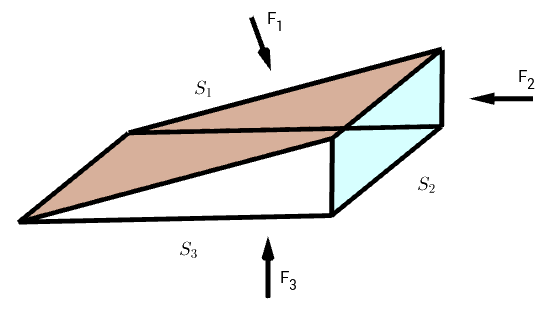
\includegraphics[width=0.4\textwidth]{Λευκάδα1.png}
 \centering
\end{figure}

Το πρίσμα ισοροπεί, άρα θα ισχύει
$$F_1 cosθ = F_3 \text{ και } F_1 sinθ = F_3$$

Αντίστοιχα λοιπόν θα ισχύει $p_1 S_1 cosθ = p_3 S_3 \Rightarrow p_1=p_3$ και $p_1 S_1 sinθ = p_2 S_2 \Rightarrow p_1=p_2$.

Αν μικρύνουμε απείρως τις επιφάνειες θα μπορούμε να ορίσουμε την πίεση σε σημείο. Από τα προηγούμενα συνεπάγεται ότι η πίεση σε σημείο είναι ανεξάρτητη της επιφάνειας που περιέχει αυτό το σημείο\textsuperscript{\cite{Feynman1}}.

\subsection{Υδροστατική πίεση}

\begin{figure}[ht]
 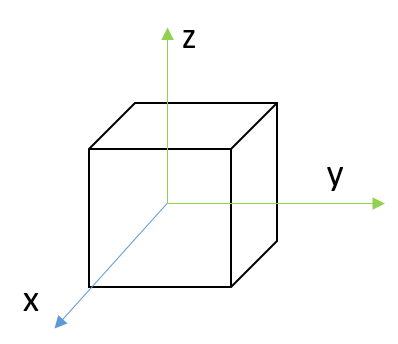
\includegraphics[width=0.3\textwidth]{Λευκάδα2.png}
 \centering
\end{figure}
Ας είναι ένας στοιχειώδης όγκος υγρού. Ο όγκος βρίσκεται σε ισορροπία, άρα όλες οι δυνάμεις που ασκούνται πάνω του έχουν συνισταμένη μηδέν. Στον οριζόντιο άξονα $y$ θα ισχύει
\begin{equation*}
 \sum F_{y} = 0 \Rightarrow F_{y1}=F_{y2} \Rightarrow p_{y1}d{\vec{A_y}}=p_{y2}d{\vec{A_y}} \Rightarrow p_{y1}=p_{y2}.
\end{equation*}
Έτσι η πίεση δεν μεταβάλεται κατά τον οριζόντιο άξονα $y$. Όμοια δείχνεται ότι $p_{x1}=p_{x2}$. Στον κατακόρυφο άξονα όμως τα πράγματα είναι διαφορετικά. Το βάρος του στοιχειώδους όγκου υγρού θα πρέπει να ισούται με την διαφορά των δυνάμεων χάρις τις πιέσεις στις αντίστοιχες επιφάνειες:
\begin{align}
 \sum F_{z} & = 0 \Rightarrow \nonumber \\ F_{z1}-F_{z2} &=B \Rightarrow \nonumber\\
 \left(p_{z_0}-p_{z_0+dx} \right)dx\,dy&=\iiint_V ρ(x,y,z)g(x,y,z)\,dx\,dy\,dz \Rightarrow \refstepcounter{equation} \label{eq:15} \\
 -dp\,dx\,dy &= ρg\iiint_V dx\,dy\,dz \Rightarrow \nonumber\\
 -dp\,dx\,dy &= ρgdz\,dx\,dy \nonumber
\end{align}

Η παραπάνω εξίσωση απλοποιήθηκε χάρις το ότι το υγρό θεωρείται ασυμπίεστο ($ρ=c$) και η επιτάχυνση της βαρύτητας είναι σταθερή σε μεταβολή ύψους $dz$. Έτσι ισχύει η \textit{υδροστατική εξίσωση}:
\begin{equation} \label{eq:13}
 \frac{dp}{dz}=-ρg
\end{equation}
Με απλή ολοκλήρωση όταν $g=-G\dfrac{M_γ}{z^2}$
\begin{gather*}
 \frac{dp}{dz}=-ρg \Rightarrow p-p_0=-ρ\int_{z_1}^{z_2} g\, dz \Rightarrow p-p_0=-ρ\int_{z_1}^{z_2} -G\frac{M_γ}{z^2}\, dz \Rightarrow \\
 p=p_0-GM_γ\left(\frac{1}{z_2}-\frac{1}{z_1}\right)=p_0+GM_γ\frac{z_2-z_1}{z_2z_1}
\end{gather*}
Αν θεωρήσουμε ότι οτιδήποτε ύψος μελετάμε είναι από το κέντρο της Γης, τότε $z_2z_1\approx R_γ^2$ και $z_2-z_1=h$. Δηλαδή
\begin{equation} \label{eq:17}
 p=p_0+G\frac{M_γ}{R_γ^2}h=p_0+ρgh
\end{equation}
από το οποίο προκύπτει ότι η υδροστατική πίεση δεν εξαρτάται από το υλικό, παρά μόνο από την πίεση στην "κάτω" επιφάνεια, το είδος του υγρού, την επιτάχυνση της βαρύτητας και το ύψος του υγρού. Με άλλα λόγια η πίεση είναι ίση σε όλα τα σημεία που βρίσκονται στο ίδιο βάθος.

Η υδροστατική πίεση λοιπόν σε μία "κάτω" επιφάνεια προκύπτει από το βάρος του υλικού (ή των υλικών) που βρίσκονται από πάνω της. Η τελευταία πρόταση είναι ίσως παρεξηγημένη, μιας και είναι το αποτέλεσμα της υδροστατικής πίεσης και όχι ο ορισμός της. Τα σχολικά βιβλία διδάσκουν την υδροστατική πίεση ξεκινώντας ότι η "άνω" επιφάνεια δέχεται δύναμη ίση με το βάρος της στήλης του νερού που βρίσκεται από πάνω της.
\subsection{Ατμοσφαιρική πίεση}
Η ατμοσφαιρική πίεση μπορεί να θεωρηθεί ως επέκταση της υδροστατικής. Η πυκνότητα όμως του αέρα αλλάζει, αφού τα αέρια συμπιέζονται. Πιο συγκεκριμένα από την υδροστατική εξίσωση $dp/dz=-ρg$ και από την καταστατική εξίσωση των αερίων
$$pV=nRT \Rightarrow p\frac{m}{ρ}=\frac{N}{N_A}RT \Rightarrow ρ=\frac{mp}{kT}$$
όπου $m$ η μέση μάζα ανά mole αερίου, $p$ η πίεση, $k$ η σταθερά του Boltzman και $T$ η θερμοκρασία, προκύπτει ότι:
\begin{equation*}
 \frac{dp}{dz}=-\frac{mp}{kT}g.
\end{equation*}
Μια περίπτωση που μπορεί να μελετηθεί στο σχολείο είναι όταν η θερμοκρασία κατά τον άξονα $z$ παραμένει σταθερή. Θα ισχύει
\begin{equation} \label{eq:16}
 \frac{dp}{dz}=-\frac{mp}{kT}g \Rightarrow \frac{dz}{dp}=-\frac{kTg}{m}\frac{1}{p} \Rightarrow z=-\frac{kTg}{m}\ln \frac{p}{p_0} \Rightarrow p=p_0e^{-\frac{m}{kTg}z}
\end{equation}

\section{Πίεση Ρευστών}
Ας θεωρήσουμε έναν οριζόντιο σωλήνα διατομής $A$ που μέσα του ρέει υγρό ασυμπίεστο, χωρίς τριβές με τα τοιχώματα. Και μόνο με την χρήση του 2ου νόμου του Newton μπορεί εύκολα να αποδειχθεί ότι $ρ\frac{v^2}{2}+p=c$, μία από τις περιπτώσεις που μαθαίνουν οι μαθητές στην Γ Λυκείου. Έχουμε:
\begin{gather*}
 F=ma \Rightarrow -Adp=ρV\frac{dv}{dt} \\
 -Adp=ρAdx\frac{dv}{dt} \Rightarrow -dp=ρv dv \\
 \frac{dp}{dv}=-ρv \Rightarrow p=-ρ\frac{v^2}{2}+c \\
 \frac{1}{2}ρv^2+p=c
\end{gather*}
Υπάρχει επίσης και η περίπτωση που ο σωλήνας δεν είναι οριζόντιος που τότε εργαζόμαστε διαφορετικά και δεν φαίνεται να υπάρχει πιο φινετσάτη απόδειξη από αυτή του σχολικού βιβλίου,
\begin{gather*}
 \frac{1}{2}ρv^2+p+ρgh=c
\end{gather*}


\begin{thebibliography}{9}
 \bibitem{fysikiB}
 \textit{Φυσική Β Γυμνασίου}.
 Ινστιτούτο Επιστήμης Υπολογιστών και Εδόσεων "Διόφαντος", ISBN: 978-960-06-2731-2, σελ. 65-66.

 \bibitem{fysikiG}
 \textit{Φυσική Γ Λυκείου}.
 Ινστιτούτο Επιστήμης Υπολογιστών και Εδόσεων "Διόφαντος", ISBN: 978-960-06-2432-8, σελ. 90-101.

 \bibitem{Halliday1}
 \textit{Fundamentals Of Physics}, Halliday, Resnick, Walker, 9th Edition, σελ. 361.
 %\url{(https://archive.org/details/FundamentalsOfPhysicsHallidayResnickWalker)}

 \bibitem{Feynman1}
 \textit{The Feynman Lectures on Physics}, Feynman, Leighton, Sands, vol. 2, ch. 40.
 %\url{(http://www.feynmanlectures.caltech.edu/II_40.html)}

\end{thebibliography}
\end{document}
